%BEGIN_FOLD packages
\documentclass[11pt]{article}
\usepackage{geometry}
\geometry{margin=1in}
\usepackage{mathptmx}
\usepackage{lipsum}
\usepackage[spanish]{babel}
\usepackage[utf8]{inputenc}
\usepackage{sectsty,textcase}
\usepackage{wrapfig}
\usepackage{ragged2e}
\usepackage{fontspec}
%\setmainfont{Arial}
%COLORES DE TITULOS
\usepackage{xcolor}
\definecolor{color1}{RGB}{12,39,50}
\definecolor{color2}{RGB}{92,92,102}
\definecolor{color3}{RGB}{230,147,32}
\definecolor{color4}{RGB}{152,152,162}
\sectionfont{\color{color1}} 
\subsectionfont{\color{color2}} 
\subsubsectionfont{\color{color3}} 

\usepackage{titlesec}
\titleformat{\section}
{\normalfont\Large\bfseries \color{color1}}{\thesection }{0.5em}{\MakeUppercase}[{\color{color3}\titlerule[1.8pt]}]
\usepackage{setspace}

\usepackage{etoolbox}
\usepackage{fancyhdr}
\usepackage{nameref}
\makeatletter
\newcommand*{\currentname}{\@currentlabelname}
\makeatother

\pagestyle{fancy}
\fancyhf{}
\usepackage{longtable}
\renewcommand\headrule{\begin{minipage}{1\textwidth}
		
	\end{minipage}\par}%
\renewcommand\footrule{\begin{minipage}{1\textwidth}
		\color{color4!30}     \hrule width  1\hsize height 1.2pt
	\end{minipage}\par}%
\lhead{ \it \color{color2!50} \MakeUppercase{\fontfamily{lmr} \normalsize \titleDocument}}
\rhead{ \color{color3!60} \fontfamily{ppl} \normalsize  \theauthor}
\lfoot{\fontfamily{lmr} \color{color3}\small \textit{\subtitle}}
\rfoot{\color{color3!90} \bfseries \thepage}
\usepackage{rotating}

%\newcommand{\date}{\today}
\usepackage{xcolor,colortbl}
\usepackage{array}
\newcolumntype{M}{>{\centering\let\newline\\\arraybackslash\hspace{0pt}}m{1.5cm}}


\usepackage{csvsimple}
\usepackage[utf8]{inputenc}
\usepackage{caption}


%BEGIN_FOLD Code_section
\usepackage{listings}
\definecolor{commentC}{RGB}{57,185,170}
\definecolor{gray}{rgb}{0.5,0.5,0.5}
\definecolor{keywordC}{RGB}{0,107,190}
\definecolor{codeBack}{RGB}{233,233,233}
\definecolor{codeBorder}{RGB}{213,203,203}

\lstloadlanguages{SQL}
\lstdefinestyle{SQLCode}{ %
	language=SQL,                  % the language of the code
	basicstyle=\small\ttfamily,       % the size of the fonts that are used for the code
	numbers=left,                   % where to put the line-numbers
	numberstyle=\tiny\color{gray},  % the style that is used for the line-numbers
	stepnumber=1,                   % the step between two line-numbers. If it's 1, each line
	% will be numbered
	numbersep=5pt,                  % how far the line-numbers are from the code
	backgroundcolor=\color{codeBack},  % choose the background color. You must add \usepackage{color}
	showspaces=false,               % show spaces adding particular underscores
	showstringspaces=false,         % underline spaces within strings
	showtabs=false,                 % show tabs within strings adding particular underscores
	frame=single,                   % adds a frame around the code
	rulecolor=\color{codeBorder},        % if not set, the frame-color may be changed on line-breaks within not-black text (e.g. commens (green here))
	tabsize=4,                      % sets default tabsize to 2 spaces
	captionpos=b,                   % sets the caption-position to bottom
	breaklines=true,                % sets automatic line breaking
	breakatwhitespace=false,        % sets if automatic breaks should only happen at whitespace
	title=\lstname,                 % show the filename of files included with \lstinputlisting;
	% also try caption instead of title
	keywordstyle=\color{keywordC} \bfseries,          % keyword style
	commentstyle=\color{commentC},       % comment style
	stringstyle=\color{color2},         % string literal style
	escapeinside={\%*}{*)},            % if you want to add a comment within your code
	morekeywords={BOOLEAN,REFERENCES,OVER,DATABASE,USE,SHOW,VISIBLE,ENGINE,IF,SCHEMA,SET,PARTITION,ROW_NUMBER}               % if you want to add more keywords to the set
}
\usepackage{listingsutf8}
\lstset{inputencoding=utf8/latin1}

% this is needed for forms and links within the text
%END_FOLD Code_section

%\usepackage[dvipsnames]{xcolor}
\usepackage{tikz}
\usetikzlibrary{ shapes.geometric }
\usetikzlibrary{calc}
\usepackage{anyfontsize}
\usepackage{caption,setspace}
\usepackage[hidelinks]{hyperref}
\usepackage{mdframed}


\usepackage{xcolor}
\newcommand\ytl[2]{
	\parbox[b]{8em}{\hfill{\color{color3}\bfseries\sffamily #1}~$\cdots\cdots$~}\makebox[0pt][c]{$\bullet$}\vrule\quad \parbox[c]{4.5cm}{\vspace{7pt}\color{color1}\raggedright\sffamily #2.\\[7pt]}\\[-3pt]}

\newcommand{\foo}{\color{LightSteelBlue3}\makebox[0pt]{\textbullet}\hskip-0.5pt\vrule width 1pt\hspace{\labelsep}}

%END_FOLD packages

%DATOS DE TITULO
\newcommand{\titleDocument}{Patrones de Arquitectura}
\newcommand{\titleDocumentComplement}{ de Software}
\newcommand{\theauthor}{García Galaz Rodolfo}
\newcommand{\authorsaffiliations}{Instituto Tecnológico de Mexicali}
\newcommand{\professor}{Jose Ramón Bogarin Valenzuela}
\newcommand{\course}{Desarrollo de Aplicaciones Móvil}
\newcommand{\subtitle}{Unidad 1}
\newcommand{\nocontrol}{20491167}
\newcommand{\location}{Mexicali, B.C.}


\begin{document}
	\captionsetup{labelfont=bf}
	%BEGIN_FOLD cover
	
	\clearpage\thispagestyle{empty}
	\justifying
	\singlespacing
	\setlength\parindent{24pt} %
	\thispagestyle{empty} %Sets the page color
	{\fontfamily{lmr}
		\begin{tikzpicture}[remember picture,overlay]
			%%%% Background
			\fill[color1!90] (current page.south west) rectangle (current page.north east);
			
			%%%% Left Bar
			\fill[color1] (1,10) rectangle (-3.5,-100);

			%%%% Left Bar
			\fill[color3] (1,10) rectangle (0.5,-100);
			
			\foreach \i in {-0.5,...,-5}
			{
				\fill[color1!98] (0.4+\i,10) rectangle (\i,-100);
			}
			
			
			%%%% Title
			\node[left,black,minimum width=0.80*\paperwidth,minimum height=3cm, rounded corners,align=center] at ($(current page.north east)+(0,-9.5)$)
			{
				{\fontsize{25}{25} \color{white} \selectfont \bfseries \titleDocument}
			};
			
			\node[left,black,minimum width=0.80*\paperwidth,minimum height=3cm, rounded corners] at ($(current page.north east)+(0,-10.5)$)
			{
				{\fontsize{25}{25} \color{white} \selectfont \bfseries \titleDocumentComplement}
			};
			
			
			%%%% Subtitle
			\node[left,black,minimum width=0.80*\paperwidth,minimum height=2cm, rounded corners] at ($(current page.north east)+(0,-11.5)$)
			{
				{\color{white} \huge \textit{\subtitle}}
			};
			
			%%%% Student Name
			\node[left,black,minimum width=0.80*\paperwidth,minimum height=2cm, rounded corners] at ($(current page.north east)+(0,-12.5)$)
			{
				{ \color{white} \Large \textsc{\theauthor}}
			};
			
			
			%%%% Student Id
			\node[left,black,minimum width=0.80*\paperwidth,minimum height=2cm, rounded corners] at ($(current page.north east)+(0,-13.5)$)
			{
				{ \color{white} \large \textsc{\nocontrol}}
			};
			
			%%%% Course
			\node[left,black,minimum width=0.80*\paperwidth,minimum height=2cm, rounded corners] at ($(current page.north east)+(0,-21)$)
			{
				{\color{white}\Large\bfseries \course}
			};
			%%%% Professor
			\node[left,black,minimum width=0.80*\paperwidth,minimum height=2cm, rounded corners] at ($(current page.north east)+(0,-22)$)
			{
				{\color{white}\Large \professor}
			};
			%%%% School
			\node[left,black,minimum width=0.80*\paperwidth,minimum height=2cm, rounded corners] at ($(current page.north east)+(0,-23)$)
			{
				{\color{white}\Large \textit{\authorsaffiliations}}
			};
			%%%%Date
			\node[left,black,minimum width=0.80*\paperwidth,minimum height=2cm, rounded corners] at ($(current page.north east)+(0,-24)$)
			{
				{\color{white}\Large \textit{\today}}
			};
			\node[left,black,minimum width=0.80*\paperwidth,minimum height=2cm, rounded corners] at ($(current page.north east)+(0,-25)$)
			{
				{\color{white}\Large \textit{\location}}
			};
			
		\end{tikzpicture}
	}
	\clearpage
	\pagestyle{fancy}
	\setcounter{page}{1}
	%END_FOLD cover
	
	\tableofcontents
	\listoffigures
	%\newpage
	\lstset{inputencoding=utf8/latin1}
	\newpage \section{Model-View-Controller}
	% TODO: \usepackage{graphicx} required
	\begin{figure}[ht!]
		\centering
		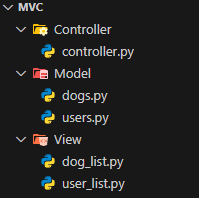
\includegraphics[width=0.3\linewidth]{img/mvc.png}
		\caption{Estructura de archivos de MVC}
		\label{fig:mvc}
	\end{figure}
	
	
		\par La estructura con el modelo MVC esta formada por las siguientes carpetas y archivos:
		\begin{itemize}
			\item \textbf{Model}. Contiene las clases de objetos y la lógica de negocios relacionada con los mismos.
				\begin{itemize}
					\item \textbf{dogs.py}: Archivo donde se declara la clase y funciones para crear, actualizar, eliminar y leer los objetos de clase Dog.
					\item \textbf{users.py}: Archivo donde se declara la clase y funciones para crear, actualizar, eliminar y leer los objetos de los usuarios.
				\end{itemize}
			\item \textbf{View}. Contiene los endpoints para el usuario final y solicita la información a través de los controladores.
				\begin{itemize}
					\item \textbf{dog\_list.py}: Muestra un listado de los perros actualmente creados en la base de datos.
					\item \textbf{user\_list.py}: Muestra un listado con los nombres de los usuarios de la base de datos.
				\end{itemize}
			\item \textbf{Controller}. Contienen las funciones para proveer a los endpoints con los datos que solicitan, y esto es a través de los modelos.
				\begin{itemize}
					\item \textbf{controller.py}: Incluye la lógica para solicitar actualizaciones, cambios, lecturas y demás a los modelos, así como el código que da formato a los datos para ser visualizados en los endpoints .
				\end{itemize}
		\end{itemize}
		
	\newpage \section{Model-View-Presenter}
		% TODO: \usepackage{graphicx} required
		\begin{figure}[ht!]
			\centering
			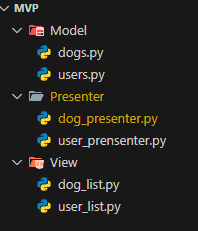
\includegraphics[width=0.3\linewidth]{img/mvp.png}
			\caption{Estructura de archivos de MVP}
			\label{fig:mvp}
		\end{figure}
		
		\par La estructura con el modelo MVP esta formada por las siguientes carpetas y archivos:
		\begin{itemize}
			\item \textbf{Model}. Contiene las clases de objetos y la lógica de negocios relacionada con los mismos.
			\begin{itemize}
				\item \textbf{dogs.py}: Archivo donde se declara la clase y funciones para crear, actualizar, eliminar y leer los objetos de clase Dog.
				\item \textbf{users.py}: Archivo donde se declara la clase y funciones para crear, actualizar, eliminar y leer los objetos de los usuarios.
			\end{itemize}
			\item \textbf{View}. Las pantallas de la aplicación y la lógica de las funciones de los elementos de la UI.
			\begin{itemize}
				\item \textbf{dog\_list.py}: Muestra un listado de los perros actualmente creados en la base de datos.
				\item \textbf{user\_list.py}: Muestra un listado con los nombres de los usuarios de la base de datos.
			\end{itemize}
			\item \textbf{Presenter}. Contienen las funciones para proveer a las pantallas con la información que necesitan en el formato que son solicitadas.
			\begin{itemize}
				\item \textbf{dog\_presenter.py}: Incluye la lógica para solicitar el listado de los objetos \textit{Dog}, así como el código que da formato a los datos para ser visualizados en las pantallas.
				\item \textbf{user\_presenter.py}: Incluye la lógica para solicitar el listado de los objetos \textit{User}, así como el código que da formato a los datos para ser visualizados en las pantallas.
			\end{itemize}
		\end{itemize}
	\newpage \section{Model-View-ViewModel}

		\begin{figure}[ht!]
			\centering
			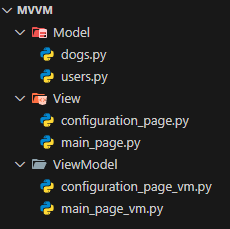
\includegraphics[width=0.3\linewidth]{img/mvvm.png}
			\caption{Estructura de archivos de MVVM}
			\label{fig:mvvm}
		\end{figure}
		
		\par La estructura con el modelo MVVM esta formada por las siguientes carpetas y archivos:
		\begin{itemize}
			\item \textbf{Model}. Contiene las clases de objetos y la lógica de negocios relacionada con los mismos.
				\begin{itemize}
					\item \textbf{dogs.py}: Archivo donde se declara la clase y funciones para crear, actualizar, eliminar y leer los objetos de clase Dog.
					\item \textbf{users.py}: Archivo donde se declara la clase y funciones para crear, actualizar, eliminar y leer los objetos de los usuarios, incluyendo funcionalidad para verificar credenciales.
				\end{itemize}
			\item \textbf{View}. Contiene el diseño de las pantallas de la aplicación
				\begin{itemize}
					\item \textbf{configuration\_page.py}: Archivo que declara la estructura visual de la página de configuración y declara como su viewmodel a su correspondiente.
					\item \textbf{main\_page.py}: Archivo que contiene la parte visual de la pantalla principal de la aplicación.
				\end{itemize}
			\item \textbf{ViewModel}. Los archivos aquí contenidos alojan la lógica funcional de las pantallas, como pueden ser las funciones de clic de cada una de las pantallas, así como las variables que contienen los valores que se muestren en las mismas.
				\begin{itemize}
				\item \textbf{configuration\_page\_vm.py}: Archivo contiene la lógica de negocios de la página de configuración y se conecta los modelos pertinentes.
				\item \textbf{main\_page\_vm.py}: Contiene la lógica de negocios de la página de principal y se conecta los modelos pertinentes.
				\end{itemize}
		\end{itemize}
	\newpage \section{Clean Code}
	
		% TODO: \usepackage{graphicx} required
		\begin{figure}[ht!]
			\centering
			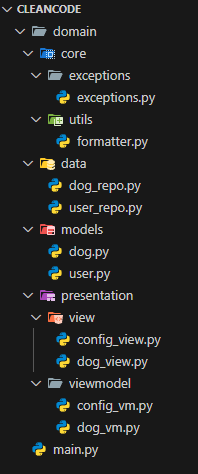
\includegraphics[width=0.3\linewidth]{img/cc.png}
			\caption{Estructura de archivos de Clean Code}
			\label{fig:cc}
		\end{figure}
		\par La estructura con el modelo Clean Code esta basada en funcionalidad y debe ser adaptada de acuerdo a la aplicación que se esta creando. El ejemplo siguiente esta basado en una aplicación en donde se muestran un listado de perros y se tiene una configuración de usuario, y por las siguientes carpetas y archivos:
		\begin{itemize}
			\item \textbf{domain}. Todo el código de la aplicación.
				\begin{itemize}
					\item \textbf{core}. Contiene funciones y demás utilizados de manera global en la aplicación como excepciones y utilerías para dar formato a múltiples pantallas. Estas funciones son generales y no especificas a una sola pantalla o parte de la aplicación.
					\item	\textbf{data}. Contiene la lógica para obtener la información de la base de datos o servicio que provee los datos que utiliza la aplicación.
					\item \textbf{models}. Contiene las clases y funciones de los objetos usados por la aplicación.
					\item \textbf{presentation}. Contiene el código relacionado con las pantallas de la aplicación
						\begin{itemize}
							\item \textit{view}: Contiene la parte gráfica de las pantallas de la aplicación.
							\item \textit{viewmodel}: Contiene la lógica de la funcionalidad de las pantallas y las variables que se muestran en la misma.
						\end{itemize}
				\end{itemize}
			\item \textbf{main.py}: Es el archivo ejecutable que inicia la aplicación.
		\end{itemize}
\end{document}
